\documentclass[a4paper,titlepage,12pt]{book}
\usepackage[suftesi]{frontespizio}
\usepackage{geometry}
\usepackage{lmodern}
\usepackage[cache=false]{minted}
\usemintedstyle{friendly}
\usepackage[italian]{babel}
\usepackage[dvipsnames]{xcolor}
\usepackage{imakeidx}[column=1, title=Indice, intoc]
\usepackage{subfig}
\usepackage{graphicx}
\definecolor{blu_pant}{RGB}{0, 64, 122}
\geometry{margin=1.2in}
\usepackage{setspace}
\setstretch{1.5}
\makeindex[columns=1, title=Indice, intoc]
\begin{document}
{\fontfamily{lmr}\selectfont
\begin{frontespizio}
\Logo{images/Universita-pisa.jpg}
\Istituzione{Università di Pisa}
\Dipartimento{Informatica}
\Corso[Laurea Triennale]{Informatica \\(classe L-31)}
\Annoaccademico{2021--2022}
\Titoletto{Relazione di Tirocinio presso l'azienda Zerynth S.R.L.}
\Titolo{\textcolor{black}{Integrazione di una piattaforma \\di veichle tracking esistente \\con l'architettura cloud di Zerynth}}
\Sottotitolo{}
\Candidato[578138]{Andrea Tufo}
\NRelatore{Tutore Aziendale}{}
\Relatore{Davide Neri}
\NCorrelatore{Tutore Accademico}{}
\Correlatore{Gabriele Mencagli}
\end{frontespizio}

\tableofcontents



\chapter{
Introduzione\index{Introduzione}}
Nell'ambito dell'Iot esistono davvero un'infinità di tipologie di dispositivi, classificati per potenza, tipologia dei dati emessi, numero, caratteristiche e tipologia dei sensori a disposizione. Tra questi ritroviamo anche dispositivi che permettono di inviare dati riguardo la loro posizione attuale, i quali si mostrano utili in innumerevoli circostanze, come ad esempio nel caso di furto o smarrimento di un veicolo, o ancora del tracciamento gps di apparecchiature militari o anche nell'ambito della mobilità, come nel caso della "micro-mobilità".\\
Questo progetto, dunque, aveva come scopo principale quello di integrare un sistema già esistente per il tracciamento veicolare chiamato "traccar"  con la piattaforma zCloud sviluppata dall'azienda Zerynth s.r.l.\\
All'interno di zCloud un utente può creare workspace, fleet e device, inoltre possono essere anche monitorati i dispositivi creati sulla piattaforma, osservando i dati che essi inviano al cloud. Il device rappresenta il \textit{digital twin} del device fisico, esso possiede degli attributi, tra i principali abbiamo un identificatore, un nome, un identificatore dell'account a cui appartiene e un identificatore relativo al fleet in cui è contenuto. Il fleet invece rappresenta logicamente un insieme di dispositivi registrati, e anch'esso possiede un identificativo ed un nome. Infine abbiamo le workspace, ovvero, degli spazi di lavoro in cui l'utente può decidere di aggiungere fleet e device.\\
La piattaforma da integrare all'interno di zCloud, traccar, è un sistema di tracciamento di dispositivi e possiede un'interfaccia grafica dove è possibile osservare il movimento real-time dei dispositivi in movimento, i suoi attributi, e dei report generati analizzando movimenti che i dispositivi hanno effettuato, e quindi vedere i viaggi, le fermate ed i percorsi tracciati dai device. Inoltre è anche possibile creare una o più geofence, ovvero delle aree limitate che l'utente può decidere di tracciare sulla mappa. Il sistema permette inoltre di ricevere delle notifiche per qualsiasi evento l'utente decida di registrarsi, come ad esempio dispositivo che entra in una geofence (o esce dalla geofence), dispositivo che inizia a muoversi o che si ferma o ancora batteria del device bassa. Anche Traccar possiede le proprie entità come ad esempio i device, i gruppi, ma a differenza di zCloud non possiede il concetto di workspace.\\
Un primo passo molto importante è stato comprendere, tramite la documentazione e tramite alcune simulazioni effettuate in ambiente docker, il funzionamento di Traccar, delle API fornite e delle funzionalità offerte dal servizio, provando ad individuare punti di forza, possibili defezioni e relazioni con l'architettura di zCloud.  \\
Dopo aver realizzato personas, use-cases e requirements, il passo seguente è stato quello di integrare Traccar con i servizi di zCloud in locale, modificando quindi il codice sorgente di traccar. Per integrare correttamente il sistema all'interno della piattaforma di zCloud, è stato necessario creare diverse interazioni con i microservizi di Zerynth, indispensabili per autorizzare e autenticare device ed utenti e accedere ai databse di zCloud in letture e in scrittura. Inoltre è stato anche essenziale apportare alcune modifiche ad un servizio di zCloud, ovvero il servizio che si occupa di gestire le diverse creazioni e modifche delle workspaces, dei fleets e dei devices. \\
Infine è stata realizzata una suite di test in python, per verificare la corretta integrazione di traccar alla piattaforma zCloud, e quindi controllare che avvenissero correttamente l'autenticazione e autorizzazione dei device, l'autorizzazione dell'utente, il salvataggio dei dati su zStorage e la creazione dei device in traccar.
\chapter{
Background e strumenti utilizzati}
Le conoscenze che ho acquisito durante il corso di studi mi hanno aiutato a comprendere le basi di partenza del lavoro che sarei andato a svolgere durante il tirocinio. Pur premettendo che buona parte degli argomenti erano quasi del tutto nuovi per me, come ad esempio la configurazione di un server nginx o l'utilizzo dei microservizi all'interno di una architettura cloud già esistente o l'utilizzo di docker e docker-compose, non ho avuto grosse difficoltà nell'apprendere tutto ciò che mi era nuovo.


{
\section{
API REST}
L'utilizzo delle API è stato fondamentale per lo svolgimento del progetto di tirocinio. Le API (application programming interface) REST (Representational State Transfer) sono molto diffuse nel mondo della programmazione web e nella realizzazione di protocolli client-server. Il sistema REST è infatti basato su HTTP e quindi si basa sulla tipologia di comunicazione client-server. In questo sistema architetturale il server espone delle API su degli entrypoint, ovvero delle url specifiche, sulle quali vengono registrate delle funzionalità in base al tipo di richiesta (post, get, put) e al tipo di parametri o payload. Il client dunque ha la possibilità di effettuare delle richieste http a queste url particolari, realizzando quindi una vera e propria chiamata di funzione remota, in quanto il server una volta ricevuta la richiesta, eseguirà la funzione che è stata registrata per quella url, con quei parametri e per quel tipo di payload. \\
In un sistema come traccar le api sono indispensabili per poter permette al client di creare nuovi devices, nuovi gruppi, eliminare entità modificarle e ottenerle dal server. Uno dei formati più utilizzati per l'invio al giorno d'oggi è il formato json (JavaScript Object Notation), un linguaggio di formattazione dei dati. Il linguaggio json è fondamentale per lo scambio client-server degli oggetti, infatti un punto di forza delle api è la possibilità del client di serializzare interi oggetti in json inviarli ad una api lato server in modo tale che il ricevente possa utilizzarli come parametri della funzione registrata a quell'entrypoint. Ovviamente anche il viceversa è una possibilità concreta, anzi molto spesso il server restituisce nella response un json, come ad esempio di un entità creata o di un report della richiesta fatta.
}





\section{
Docker e docker-compose}
Docker è una piattaforma che permette di eseguire in un ambiente sicuro applicazioni tramite codice sorgente o immagini, infatti permette di creare un \textit{container}, ovvero un contenitore nel quale è possibile eseguire uno script o più in generale del codice. Ma la vera caratteristica utile di docker, è docker-compose, ovvero la possibilità di collegare più applicazioni e quindi più container tra di loro in una network. A tutti gli effetti viene realizzata una vera e propria rete docker, in cui le applicazioni che sono in esecuzione su essa possono comunicare tra loro scambiandosi dati e informazioni.\\
Ogni servizio di una rete di docker-compose ha essenzialmente due file principali: il docker-compose.yml ed il Dockerfile. Il primo è in pratica un insieme di regole che quel servizio deve seguire o prima di avviare la propria esecuzione o durante la propria esecuzione, come ad esempio le porte che deve esporre, l'hostname all'interno della rete docker o anche le dipendenze che ha nei confronti degli altri servizi. Il Dockerfile presente anche in docker, è paragonabile ad un makefile, ovvero una sequenza di comandi che il sottosistema con kernel linux simulato deve eseguire per avviare il servizio, che può essere uno script ad esempio o un intero apparato applicativo.\\
Docker infatti è a tutti gli effetti un sistema virtuale, e come tale è implementata una simulazione di un kernel Linux, sulla quale vengono eseguiti in modo del tutto isolato i diversi container.
Per far questo docker isola a livello di sistema i container limitando risorse come per esempio la CPU o quantità di memoria usufruibile da un container, rendendo così ogni servizio indipendente dagli altri a livello di risorse utilizzate. Docker riesce a far ciò utilizzando librerie per interfacciarsi con il sistema linux ed utilizzare funzionalità come namespace che offre la possibilità di limitare ciò che un processore o un insieme di processori può vedere a livello di informazioni relative, ad esempio, agli utenti come il loro Id, e cgroup che permette di associare ad un gruppo di processi delle limitazioni di risorse hardware (quantità di CPU, memoria, rete) e software (permessi alle risorse).


\subsection{
Utilizzo di docker e docker-compose}
Questi due strumenti li ho entrambi utilizzati in primis nella simulazione che ho effettuato per studiare il sistema ed il funzionamento di Traccar e delle sue API e successivamente per implementare e testare l'integrazione di Traccar con i microservizi di zcloud all'interno della architettura cloud in locale. \\
Una volta scaricati i servizi di zerynth infatti, lanciando l'esecuzione di un programma utility è possibile avviare una rete docker-compose locale, composta dalle immagini dei servizi reali presenti all'interno dell'architettura cloud, e dai servizi sviluppati in locale\footnote{Nel mio caso in locale ho sviluppato \textit{traccar-service} e anche \textit{wfd-service}, in quanto ho dovuto apportare delle modifiche a questo servizio di zerynth.}
All'interno dell'architettura erano presenti alcuni servizi come "portainer" che permette di visualizzare graficamente i container, i logs di ogni container, ed è stato un utilissimo strumento di debug. Oltre a portainer, è possibile citare tra i servizi principali che presentano un ambiente grafico, "pgadmin" per monitorare il database in postgres e "rqm" che permette di visualizzare lo stato delle code rabbitMQ.


\section{
Code rabbitMQ}
Durante la fase centrale del progetto ho dovuto affrontare la parte relativa alla gestione dei dati inviati dai device tracciabili a Traccar, e pertanto mi sono servito dell'utilizzo delle code rabbitMQ per poter salvare i dati sullo storage di zCloud.
Le code rabbitMQ non sono altro che un ausilio per realizzare la struttura publish-subscribe del protocollo MQTT. Questa tipologia di protocolli è definita da tre entità, Un publisher, un broker ed un subscriber. Il subscriber si registra a dei "topic" per i quali è intenzionato ricevere dei dati, il publisher, invece, pubblica all'interno di "topic", il broker infine si occupa di gestire le comunicazioni che avvengono, e dunque, strutturalmente parlando si colloca al centro tra i subscriber e i publisher. Ogni coda rabbitMQ rappresenta un topic sul quale i device pubblicano, o meglio, ogni coda possiede una "binding-key" (o routing-key) ovvero una chiave univoca che la identifica.
In realtà il funzionamento delle librerie di rabbitMQ è leggermente diverso ed un po' più complesso.\\
Partiamo col dire che una coda rabbitMQ possiede come entità un \textit{publisher} che pubblica i dati su una coda, ed un \textit{consumer} che prende i dati dalla coda a cui è inscritto. Inoltre è presente un'ulteriore entità, l'\textit{exchange}, che rappresenta un intermediario tra il publisher e la coda. L'exchange ha il compito di scegliere come e dove pubblicare il dato ricevuto dal publisher secondo un algoritmo specifico. Le tipologie di algoritmi principali sono tre: \texttt{fanout} che permette di inviare dati a tutte le code presenti, \texttt{direct} che inoltra il dato solo alla coda alla quale viene indicato il topic del publisher, e poi abbiamo la tipologia \texttt{topic}. Nel mio caso la tipologia era quella di un exchange topic, ovvero molto simile alla tipologia direct ma con la differenza che in questo caso le routing-key non hanno una qualsiasi struttura, bensì sono costruite in un modo specifico, ovvero essa è rappresentata come una lista di "tag", come se fosse una URI, ma con i punti a delimitare le parole, ad esempio \textit{j.data.dev-87y.temp}.
E' bene specificare che mentre il publisher ed il subscribe rappresentano delle entità che devono essere implementate, l'exchange è un oggetto che già esiste, è necessaria esclusivamente la sua configurazione.\\
Nel mio caso specifico ho utilizzato le librerie di java per rabbitMQ, ed una volta individuato il punto del codice sorgente di Traccar in cui viene gestita la comunicazione con i device, ho implementato un publisher che pubblica i dati, che traccar aveva ricevuto poco prima dal device, su una coda rabbitMQ presente sul cloud di zerynth.\\
L'exchange in zCloud era nominato \textit{amq.topic}, mentre la binding key era nominata \textit{data}. L'intero sistema per inviare i dati dei device alle code rabbitMQ, è stato realizzato in modo tale che i device comunicassero i propri dati al server di traccar, il quale, dopo aver eseguito l'autenticazione e l'autorizzazione del dispositivo sfruttando microservizi interni allo zCloud, invoca l'esecuzione di un metodo presente all'interno di una classe, realizzata per gestire le interazioni con i vari servizi di zCloud, detto \texttt{publishOnRMQ()} in cui viene effettuata la scrittura sulla coda precedentemente indicata con il tag \textit{latlon}, che indica un dato relativo alla posizione del device. Infatti viene memorizzato un vero e proprio file json che corrisponde al marshalling di un entità detta \texttt{Position} presente in Traccar.
\chapter{
Studio del sistema e analisi dei requisiti}
La prima parte del tirocinio era composta da due fasi, ovvero uno studio preliminare della piattaforma, e dunque comprendere quali erano le entità coinvolte, come erano fatti gli oggetti che Traccar creava e gestiva (user, device, gruppi) e soprattutto uno studio mirato alle API fornite da Traccar stesso; la seconda fase invece è consistita nel trovare un parallelismo tra le entità di Traccar e le entità di zCloud, discutendone analogie, differenze e similitudini, e successivamente pensare a come si sarebbe potuto costruire il workflow di un utente generico che intendesse aggiungere su zCloud un device tracciabile, definendo quindi personas, user stories, use cases e requirements.\\

\section{
Studio della piattaforma Traccar}
Per comprendere al meglio le funzionalità che Traccar offriva, dopo aver analizzato la documentazione, ho realizzato una simulazione utilizzando docker e docker-compose.\\
La simulazione era composta da una immagine di Traccar, un database postgres, e un client scritto in go che utilizzasse la maggior parte delle api fornite da Traccar. Il client infatti era diviso in una fase di inizializzazione in cui eliminava tutti gli oggetti creati da un'eventuale esecuzione precedente e successivamente in una fase di inizializzazione dell'ambiente e quindi con la creazione dei devices dei groups e delle altre entità che Traccar offre.\\
Da questo studio delle API di Traccar sono emersi tutti i punti di forza e tutte le criticità di Traccar, e qui di seguito proverò a riassumerle in modo da capire meglio quali sono le problematiche che io ed il mio tutore aziendale abbiamo dovuto affrontare durante il corso del tirocinio.

\subsection{
Come funziona Traccar}
La piattaforma da integrare ha essenzialmente la tipica struttura di una web-application, costituita da un server, più precisamente un Jetty Web Server, che espone delle API e le websocket, un client e un database. Il server si occupa di gestire tutte le richieste dei vari client che interagiscono con esso tramite web app, mentre le connessioni con i devices sono gestiste da una Netty network pipeline che comunica indirettamente con il web server.\\
Questa piattaforma supporta molteplici tipi di protocolli per quanto riguarda i device e nel caso ad esempio della mia simulazione ho utilizzato il protocollo OSMand (OpenStreetMap Automated Navigation Directions) poiché è davvero semplice da rispettare ed applicare. I device infatti pubblicano la loro posizione e i loro attributi direttamente al server utilizzando il protocollo scelto, compreso il loro uniqueId tramite il quale il sistema riesce ad identificare univocamente il device fisico associato al suo digital twin. Il database di default di Traccar è utilizzabile solo per quanto riguarda la fase di testing, mentre è consigliabile, da quanto riportato dalla documentazione di traccar di utilizzare un database esterno per la fase di sviluppo.    
\newpage

\begin{center}
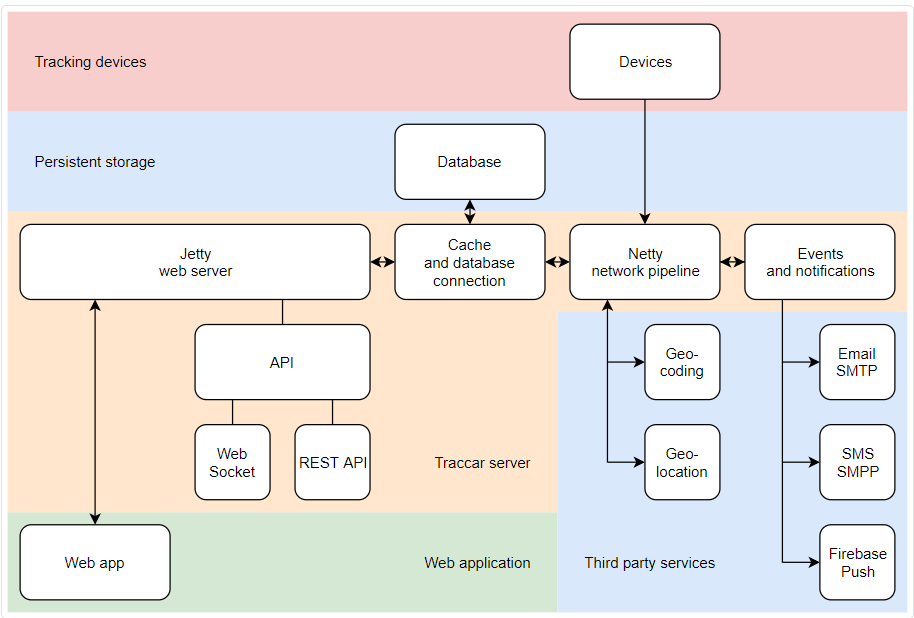
\includegraphics[scale=0.7]{images/arcTraccar.png} \\
\textit{Figura 3.1.1: Architettura di traccar}
\end{center}

\subsection{
Analisi statica del codice di traccar}
Sebbene questa parte non sia stata realizzata in un ordine cronologico definito, bensì è stato un processo che ho eseguito durante tutto il corso del progetto, è necessario descrivere in generale come è costituito il codice di traccar in modo da poter comprendere al meglio le sezioni successive di questo documento.\\
Il codice di traccar, in particolare lato server, è costituito da più parti divise in directory che svolgono ruoli differenti. Abbiamo la directory \texttt{api} e \texttt{api/resource} dove sono registrati tutti gli entrypoint delle api di traccar. Poi tra le directory più importanti abbiamo i \texttt{models} dove si trovano tutte le classi che rappresentano gli oggetti presenti in traccar, come ad esempio devices, groups e geofences e la directory \texttt{protocols} che contiene tutti gli algoritmi di decodifica di tutti i protocolli supportati da traccar. Abbiamo inoltre la directory \texttt{handler} dove sono contenuti tutte le classi che hanno il compito di handling di eventi come un device che inizia ad inviare dati al server o una notification da inviare al client. Infine è importante citare anche la directory \texttt{database}, dove si trovano tutte le classi che gestiscono i dati, e quindi forniscono tutti i metodi necessari per interfacciarsi al database di traccar a seconda dell'entità desiderata, e quindi abbiamo ad esempio il \texttt{DeviceManager()} che gestisce i dati riguardanti i device e così via. Infatti in questa directory è presente una classe detta \texttt{DataManager()} in cui sono eseguite le query necessarie per inserire, prelevare e modificare i dati dal database.


\subsection{
 Architettura di zCloud}
L'architettura del cloud di Zerynth è composta da tanti microservizi che cooperano per svolgere azioni e funzionalità specifiche. Nel mio caso ho dovuto spesse volte interfacciarmi con molti di questi microservizi per poter accedere ad esempio ai database di zerynth sia in scrittura che in lettura. \\
Giusto per citarne alcuni: \textit{rpgboucer}, \textit{login-service}, \textit{wfd-service}, \textit{dev-authorization-service}, \textit{dev-authentication-service}. Il primo permette di accedere solo in lettura ad un particolare database di Zerynth chiamato \textit{zStorage}\footnote{
I database in zerynth sono principalmente tre zCloud, ZDM e zStorage, nell'ultimo in particolare vengono memorizzati per ogni workspace tutti i dati pubblicati dai device.} composto a sua volta da sei partizioni, tre dette "master" e tre "repliche" dei relativi master.\\
Il servizio di login-service permette di autorizzare un utente registrato, e nel mio caso ho utilizzato questo servizio indirettamente, e più avanti nel documento verrà spiegato meglio nel dettaglio.\\
In seguito abbiamo il wfd-service che in realtà ho dovuto modificare, in quanto questo servizio gestisce la creazione, l'aggiornamento e la rimozioni delle entità all'interno dello zCloud, ed infine i servizi dev-autentication e dev-authorization, indispensabili per l'autenticazione del device e per autorizzare quest'ultimo ad utilizzare le risorse all'interno dell'architettura di zerynth.

\subsection{
Caratteristiche di Traccar}
Traccar offre una caratterizzazione del proprio spazio di lavoro (anche se come vedremo dopo non esiste in realtà il concetto di "workspace" di un utente), infatti si ha la possibilità di aggiungere una "geofence" per limitare un'area specifica che può essere realizzata con qualsiasi tipo di forma, delle "notifications" per ricevere delle notifiche sugli eventi a cui si è interessati, aggiungere dei "commands" ovvero degli attributi calcolati sulla base degli attributi base che un device possiede. Inoltre un'altra cosa di rilievo è senza dubbio poter personalizzare ogni singolo device aggiungendo un set potenzialmente infinito di attributi custom. Da segnalare anche la possibilità di poter usufruire dei reports personalizzabili e anche di grafici riguardanti i device associati ad un profilo. \\

\subsection{
Problematiche emerse}
Purtroppo sono emerse diverse problematiche durante il corso del progetto e molte scelte effettuate in fase di analisi sono state modificate in quanto nelle fasi più mature del progetto è migliorata la consapevolezza degli strumenti e la conoscenza del codice stesso di traccar. \\
Una delle problematiche più importanti è certamente la mancanza di accedere al servizio da terze parti utilizzando dei token d'accesso. O meglio, è possibile estendere le funzionalità di traccar per l'autenticazione in modo tale da sfruttare il protocollo LDAP per l'autenticazione da terze parti. Nonostante ciò, questa ipotesi è stata scartata in quanto poco pratica da realizzare, la strada presa è stata quella di estendere direttamente il codice sorgente di traccar.\\
Inoltre anche il claiming del dispositivo è stato un passo importante da realizzare in quanto traccar non supporta l'utilizzo di token firmati da parte dei device, bensì l'autenticazione dello stesso è effettuata solo tramite l'analisi del codice IMEI del device.

\section{
Entità di zCloud}
zCloud ha un'impostazione leggermente diversa da Traccar, in quanto permette di creare per ogni utente diversi spazi di lavoro, ma nonostante ciò alcuni oggetti sono molto similari. In zCloud ogni utente ha la possibilità di creare da una a più workspace, in ogni workspace da zero a più fleet e in ogni fleet da zero a più device. Analizzeremo adesso la struttura dei json di ogni elemento di zCloud, confrontandola con quella dell'oggetto che ho deciso di mappare in Traccar.


\section{
Parallelismo Traccar e zCloud}
In questa fase era necessario trovare delle soluzioni adeguate per quanto riguarda la comparazione delle classi, tra quelle di traccar e quelle di zCloud. Bisognava quindi trovare una relazione tra le varie entità e capire come codificare un oggetto presente in zCloud in uno di Traccar nel modo migliore possibile. Come vedremo qui di seguito il problema più grande sarà rappresentato dalla workspace, entità che in zCloud esiste, al contrario di traccar.



\paragraph{
Device}
Il device in zCloud ha una forte similarità con il device in Traccar, qui di seguito presento il json dell'oggetto di Traccar a quello di zCloud.\\



\begin{center}

\begin{tabular}{c c c c}

    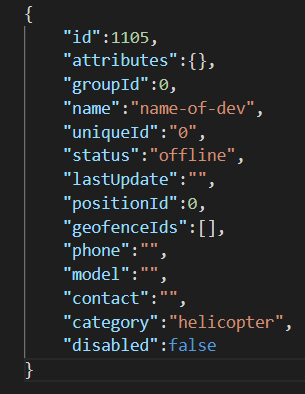
\includegraphics[scale=0.8]{images/traccDev.png}


 &  
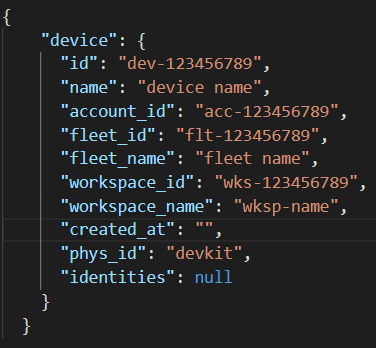
\includegraphics[scale=0.6]{images/zClDev.png} \\
\textit{Fig. 3.3-1: Device in Traccar} &  \textit{Fig. 3.3-2: Device in zCloud}
\end{tabular}
\end{center}\par\medskip


Abbiamo infatti una corrispondenza quasi uno a uno con molti attributi, quali ad esempio \textit{id}, \textit{name}, che sono ovvie ed intuitive. Inoltre anche attributi come il \textit{fleet\_id}, il \textit{workspace\_id} ed il \textit{pyhs\_id} in zCloud hanno una corrispondenza implicita ma che comunque esiste. Tratterò l'argomento della workspace in seguito,  perciò adesso mi concentrerò sul \textit{fleet\_id} e sul \textit{phys\_id}. Il primo può essere perfettamente mappato con il \textit{group\_id}, poiché come vedremo successivamente, il fleet è simile al group di Traccar,il \textit{pys\_id} invece è in relazione con lo \textit{uniqueId} essendo entrambi due identificatori univoci del dispositivo fisico. Infine \textit{account\_id} in zCloud può essere in realtà ignorato dato che ogni dispositivo in Traccar è collegato al suo user, in quanto osservando lo schema relazionale, esiste un collegamento tra la tabella degli user e quella dei device.\\
Per i restanti attributi, nel caso in cui dovessero essere necessari, si può ricorrere alla creazione di nuovi attributi nell'entità device di Traccar, utilizzando il tag \textit{attributes}.

\paragraph{
Fleet}
Per quanto riguarda i fleet, come già accennato in precedenza, ho trovato una relazione con il group di Traccar, qui di seguito, nelle figure 3.3-3 e 3.3-4, il confronto con i due json degli oggetti.




\begin{center}

\begin{tabular}{c c c c}

    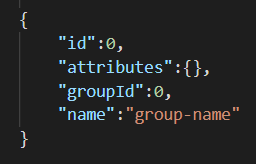
\includegraphics[scale=0.8]{images/traccGr.png}

    \label{fig:my_label}

 &  
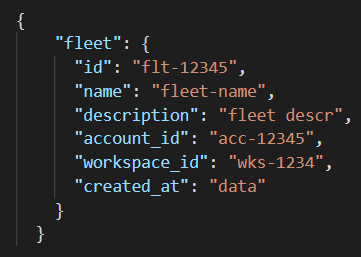
\includegraphics[scale=0.7]{images/zClGr.png} \\
\textit{Fig. 3.3-3: group in Traccar} &  \textit{Fig. 3.3-4: Fleet in zCloud}
\end{tabular}
\end{center}\par\medskip


Vale anche qui il discorso fatto per i device, si vede chiaramente come le due entità sono molto simili. E' importante evidenziare che nell'entità del group di  traccar ci sia anche un \textit{groupId} da non confondere con l'\textit{id}, in quanto il primo indica l'indice del gruppo parent a cui appartiene, infatti in Traccar un gruppo può avere infiniti sottogruppi a cui fa da parent. 

\paragraph{
Workspace}
Terminando l'analisi con la workspace, dopo aver pensato a diverse idee su come modellarla in Traccar, la soluzione che scelta è stata quella di mapparla come un group che non ha parent. Una workspace quindi è a tutti gli effetti un gruppo che ha l'\textit{groupId} sempre a zero, in quanto non appartiene a nessun gruppo. Tutti i suoi gruppi figli invece, faranno essenzialmente le veci dei fleet.\\
Grazie a questa caratteristica di Traccar, ovvero che l'entità del group è qualcosa di generico, che rappresenta un inseme di elementi eterogenei, è stato possibile mappare con successo anche la workspace di zCloud, come rappresentato graficamente nelle figure 3.3-5 e 3.3-6.


\begin{center}
\begin{tabular}{c c c cc c c}


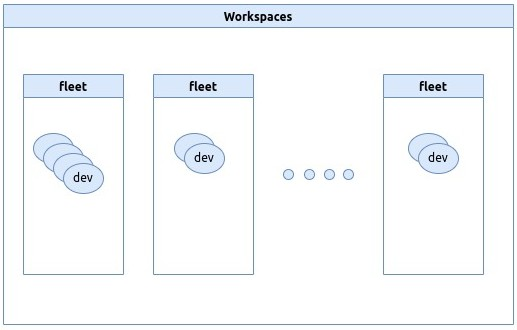
\includegraphics[scale=0.6]{images/wks.jpg}\\ 
\textit{Fig. 3.3-5: Workspace di zCloud}\\
\\
\\
\\
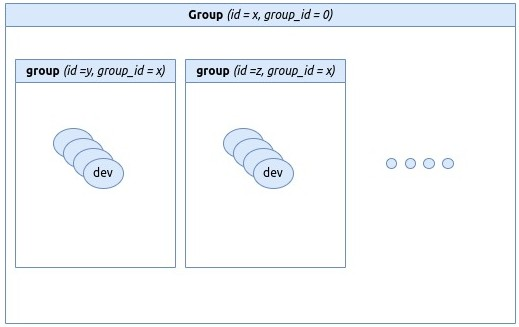
\includegraphics[scale=0.6]{images/groups.jpg} \\
\textit{Fig. 3.3-6: Workspace mappata in group in Traccar}

\end{tabular}
\end{center}

\section{
Personas e requisiti}
l'Ultimo passo prima di iniziare l'implementazione e l'integrazione effettiva del servizio traccar, è stato quello di descrivere alcuni archetipi di potenziali utilizzatori del servizio e quindi successivamente definire i possibili requirements.\\
In questa fase ho analizzato tre personas di cui due di queste appartenenti al mercato B to B e una sola personas che svolgeva il ruolo di consumer normale. Le aziende che potrebbero voler usufruire di questo servizio possono quindi essere legate al mondo dei trasporti, all'ambito militare o nel noleggio di veicoli come ad esempio tutte quelle realtà che si occupano di micromobilità.\\
Prima di passare ai requisiti ho descritto alcuni use cases, azioni che l'utente potrebbe potenzialmente svolgere sul sistema in sviluppo. Prendendo ad esempio la creazione di un device tracciabile di un utente già registrato su zCloud, in figura 3.4 è rappresentato lo schema relativo di questa attività.

\begin{center}
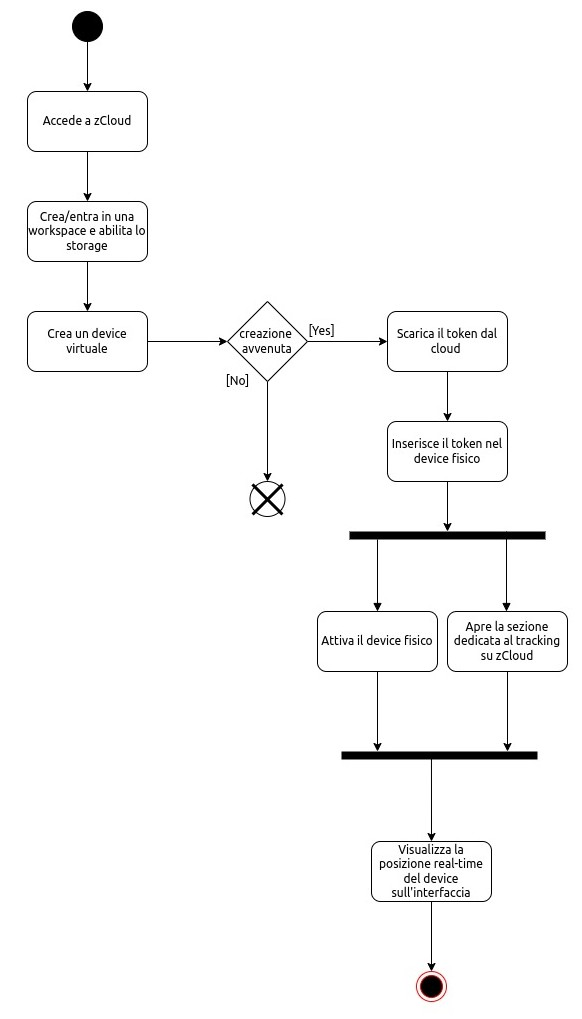
\includegraphics[scale=0.42]{images/diagramma.jpg}\\ 
\textit{Figura 3.4: Diagramma dell'attività di un utente sulla creazione di un device e la sua visualizzazione della posizione real-time su interfaccia}\\
\end{center}

\pagebreak
E quindi sono infine passato ai requisiti tra i quali abbiamo ad esempio:
\begin{itemize}
\item L'utente non può aggiungere lo stesso device tracciabile due volte;
\item Una workspace abilitata a tracciabile può contenere solo device tracciabili;
\item Una workspace non abilitata a tracciabile non può avere device tracciabili;
\item L'utente può avere lo stesso device su due o più workspace.\\
\end{itemize}

Terminata a questo punto la parte iniziale, non ci resta che procedere con la descrizione dell'integrazione effettiva della piattaforma, che, come sarà descritto nel capitolo successivo, è stata realizzata basando il lavoro sulle analisi preventive che ho presentato poco fa, nonostante la conoscenza di traccar e del suo funzionamento è naturalmente diventata sempre più accurata e approfondita man mano che il progetto prendeva forma.


\chapter{
Integrazione del sistema}
Inizialmente era necessario poter accedere ai servizi di zerynth, e per fare ciò ho scaricato, tramite la repository aziendale, la loro architettura in locale, seguendo una determinata procedura che mi ha permesso di ottenere tutte le immagini dell'architettura di zerynth e di conseguenza inserire il codice sorgente di traccar come servizio proveniente non da un'immagine bensì da una vera e propria build del codice del software, modificando alcuni file di configurazione che avevano spesso il formato di file ".yml".\\
Per integrare correttamente il sistema di Traccar con la piattaforma di zerynth, è stato necessario mettere in collegamento il servizio di tracciamento dei dispositivi con i microservizi interni dell'architettura cloud di zCloud. E' stato dunque fondamentale capire come realizzare le chiamate api agli entrypoint che i servizi di Zerynth esponevano e codificare i dati ottenuti da essi per poi poterli utilizzare correttamente. \\
La fase iniziale dell'intero processo di implementazione è consistita nell'inserire traccar all'interno dei servizi di zCloud, connettendo il servizio all'intera architettura. Per far ciò ho dovuto implementare un flie di configurazione di traccar e inserirlo nell'apposita directory, nella quale era situata tutta la configurazione di NGNIX, il proxy-server di zCloud. Successivamente è stato necessario autenticare l'utente attraverso l'account id che il \textit{login-service} di zCloud inviava come response nel caso in cui una autenticazione di uno user fosse andata a buon fine, e poi passare anche all'autenticazione e autorizzazione dei device che avrebbero dovuto poi comunicare con traccar. \\
Ovviamente per poter testare (ovviamente inizialmente tutto in locale) le singole fasi di implementazione, era necessario avvalersi di una simulazione di un device che invia dati fittizzi al servizio traccar. Per far ciò ho realizzato un piccolo script in golang che invia dati al sistema utilizzando il protocollo OsmAnd \footnote{OsmAnd (OpenStreetmap Automated Navigation Direction protocol) è un protocollo di live tracking utilizzato dall'omonimo software di tracciamento OsmAnd, esso si può impiegare, lato device, inserendo nella url, alla quale il dispositivo intende mandare i dati, tutti i parametri necessari alla localizzazione e identificazione del device stess. Un esempio di url strutturata in base al protocollo OsmAnd è il seguente: "http://tracking.org:5023/?id=23\&lat=34.4\&lon=2.4\&speed=0\&alt=2345"}(scelta esclusivamente per una questione di praticità, il protocollo OsmAnd è molto semplice da realizzare) simulando quindi gli spostamenti di un dispositivo che si muove sulla mappa.

\section{
Configurazione di Traccar in NGNIX}
In questa parta ho realizzato il primo collegamento con traccar e la struttura di zCloud, collegando il servizio al proxy-server. Oltre a specificare il dominio con il quale Traccar sarebbe diventato raggiungibile dagli host esterni all'architettura di zCloud, la connessione ad NGNIX permette alla piattaforma di delegare le operazioni di default al cloud e quindi ai microservizi interni. Ad esempio, una delle principali azioni che in parte viene delegata ad uno dei servizi di Zerynth è l'autenticazione dello user quando intende accedere a traccar. \\
NGNIX infatti inoltra la richiesta di login da parte di un utente ad un servizio chiamato \textit{login-service}, il quale si occupa di verificare l'esistenza di tale utente, e nel caso in cui l'autenticazione andasse a buon fine login-service restituisce un parametro al proxy-server, ovvero l'account id dell'utente appena verificato. NGNIX dunque inserisce questo identificativo all'interno di un campo dell'header, così da poter permettere a tutti i servizi interni di identificare l'autore delle richieste interne che si scatenano in cascata, come mostrato graficamente in figura 4.1.

\begin{center}
\centering
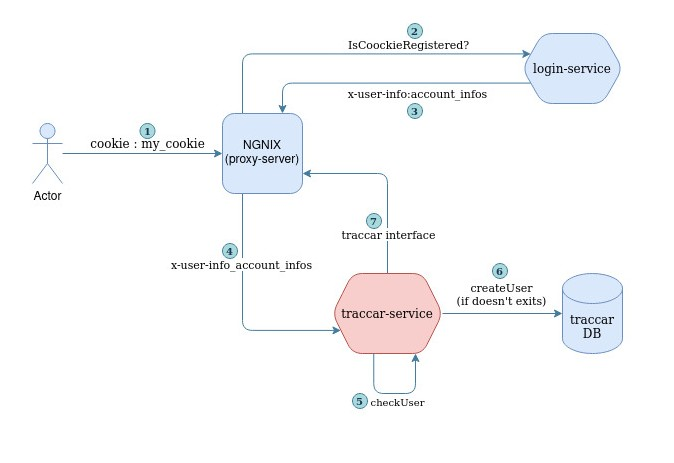
\includegraphics[scale=0.6]{images/traccar_login_serv.jpg}\\ 
\textit{Figura 4.1: Prima fase di integrazione di traccar}\label{fig:}

\end{center}

Per completare la configurazione di traccar con NGNIX era fondamentale inserire anche l'inoltro delle connessioni per le web-socket, in quanto i client si connettono ad esse per aggiornare i dati riguardanti i device e in generale le entità presenti. Pertanto ho dovuto inserire una nuova location \texttt{/api/socket} in cui venivano inoltrate tutte le richieste effettuate a \texttt{http://traccar-service:8082/api/socket}.


\section{
Autenticazione dell'utente in Traccar}
Il normale funzionamento di traccar prevede un login composto da username e password per accedere al servizio. Ma questa soluzione non era naturalmente adeguata al nostro scopo, era infatti necessario poter far accedere l'utente automaticamente una volta che si fosse registrato e avesse effettuato l'accesso su zCloud. In realtà buona parte di questa funzionalità era già realizzata in quanto il cloud possiede un servizio che autentica lo user, citato in precedenza il \textit{login-service}. Questa piccola parte architetturale funziona nel seguente modo, seguendo lo schema in figura 4.1:\\
\begin{enumerate}
\item Il proxy-server NGNIX riceve la richiesta di accesso da parte di un client all'url in cui traccar è specificato come location (ad esempio traccar.zerynth.localhost) con il cookie dell'utente;
\item NGNIX inoltra la richiesta al \textit{login-service} con il cookie che l'utente ha passato nella richiesta precedente;
\item Il servizio restituisce al server NGNIX la risposta, nella quale se l'utente risulta esistere, viene incluso l'account-id di tale utente all'interno di un campo header \textit{x-user-info};
\item NGNIX inoltra poi la richiesta iniziale, con l'aggiunta del nuovo campo dell'header a traccar;

\item All'interno del \textit{traccar-service} viene eseguito un controllo per verificare che l'utente con quell'account-id sia già registrato nel database di traccar, se così dovesse essere viene inviata l'interfaccia al proxy-server che la restituisce al client, altrimenti prima di inoltrare l'interfaccia ad NGNIX, viene creato un nuovo utente in traccar e salvato nel database di \textit{traccar-service}.
\end{enumerate}


\subsection{Implementazione in traccar}
Focalizzando l'attenzione solo sul servizio traccar, è stata implementata la funzionalità che garantisce la corretta autenticazione dell'utente, all'interno di una classe denominata \texttt{SessionResource()}. Questa classe gestisce le richieste all'entrypoint\footnote{Per entrypoint si intende l'api esposta dal server, ovvero la parte di url che aggiunta alla base url del server garantisce delle funzionalità registrate, ad esempio nell'api \texttt{traccar.zerynth.localhost/api/session}} \texttt{/api/session}, in cui di norma ha il seguente formato:\par\medskip

\begin{center}\begin{flushleft}
HOST: "http://traccar\_url/api/session"\\
HEADER: "Authorization Basic: user\_code64:password\_code64"\par\medskip
\end{flushleft}

\end{center}

Perciò la modifica che ho apportato a questa classe è stata quella di poter reperire il campo \texttt{X-USER-INFO} dell'header della richiesta, ottenere l'account-id, e verificare l'esistenza di utente che ha il campo "name" uguale all'account-id in questione. Se dovesse esistere già un utente allora viene restituita correttamente la sessione al client, inoltrando come payload in formato Json, i dati relativi all'utente stesso. Altrimenti, se l'utente non è presente in traccar, viene creata una nuova istanza e salvata nel database. La richiesta accettata, proveniente da NGNIX sarà quindi così formata:
\par\medskip

\begin{center}\begin{flushleft}
HOST: "http://traccar\_url/api/session"\\
HEADER: "Authorization Basic: user\_code64:password\_code64"\\
\qquad \qquad \quad       "X-USER-INFO" : acc\_infos
\end{flushleft}

\end{center}
\subsection{
Considerazioni sulla soluzione}
Possono essere effettuati dei miglioramenti e delle ottimizzazioni a questa soluzione, ad esempio evitando di duplicare l'entiotà nel database di traccar. La scelta è stata quella di tenere questa implementazione in quanto essa rappresenta una realizzazione pratica e funzionale, infatti, uno dei problemi che avremmo dovuto affrontare se l'entità utente non fosse salvata nel database di traccar, sarebbe stato quello di mantenere tutti i link con gli oggetti come le geofence e le notification, ovvero tutti quegli oggetti che obbligatoriamente appartengo allo schema relazionale di Traccar. Più avanti vedremo come ho effettuato alcuni tentativi per evitare lo "sdoppiamento" delle risorse e quindi ad esempio avere per uno stesso device un'istanza sul database di traccar e un'altra sul database di zCloud.


\section{
Gestione della comunicazione con i device}
I device che comunicano con traccar-service possono essere tanti e di diversa tipologia. In questa parte vederemo come traccar gestisce la comunicazione con i dispositivi, autenticandoli, autorizzandoli e salvando i dati che inviano nel database.\\
Il device comunica direttamente con il servizio di traccar, viene autenticato, e quindi viene verificata l'esistenza di tale device, e poi autorizzato ad utilizzare le risorse che il cloud mette a disposizione come ad esempio il salvataggio dei dati. Una volta autenticato ed autorizzato correttamente, indipendentemente dal tipo di protocollo che il device usa, traccar decodifica i dati attraverso dei decoder di protocolli, creando un oggetto di tipo \texttt{Position}. Il Json di questo oggetto viene salvato sullo zStorage di zCloud, in modo tale da permettere anche ad altri servizi all'interno dell'architettura dell'azienda di poter accedere a quei dati, senza dover modificare altri servizi.\\
In generale si può schematizzare tutta la parte relativa ai dispositivi in una sequenza di azioni svolte da traccar, ecco qui di seguito una rappresentazione di questa parte architetturale che comprende solamente la parte di autorizzazione, autenticazione e memorizzazione dei dati.

\begin{center}

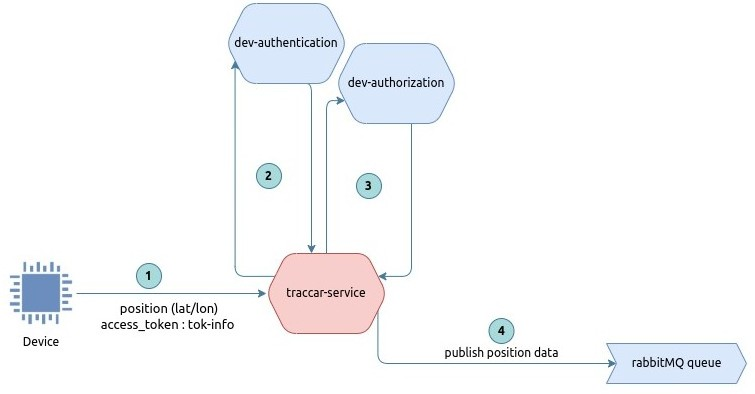
\includegraphics[scale=0.6]{images/dev-aut-traccar.jpg}\\ 
\textit{Figura 4.3: Integrazione dei device tracciabili}
\end{center}

\subsection{
Autenticazione e autorizzazione dei device}
Quando un device invia dei dati al sistema tramite uno dei protocolli che traccar supporta, le prime azioni che traccar deve effettuare sono autenticare e autorizzare\footnote{
Per \textit{autenticazione} si intende la verifica da parte di dev-authentication che il device esista correttamente per quell'user specifico. Mentre per l'\textit{autorizzazione} il dev-authorization si occupa di assicurarsi che il device abbia i diritti necessari di lettura e/o scrittura all'interno della piattaforma.} il dispositivo, solo a quel punto può effettuare il salvataggio del payload all'interno di zStorage.\\
Per l'autenticazione è stato necessario contattare il dev-authentication service di Zcloud inviando come payload un file Json specifico che contenesse precise informazioni riguardanti il device che dev'essere autenticato. Traccar riceve il device\_id e l'access-token del dispositivo dal dispositivo stesso \footnote{
L'\textit{access-token} viene generato dal cloud ed attribuito al device per poter identificare univocamente lo stesso in fase di autenticazione.} e con queste due informazioni costruisce il payload da inoltrare al servizio di Zerynth. Il Json specifico da inviare come payload è rappresentato qui sotto.


\begin{minted}{json}
{
   "client_id":"dev-9dozztcisbhj",
   "entity":"dev-9dozztcisbhj",
   "token":"bsbhJonvdTVFgvkBH98JJKnbkl",
   "proto":"mqtt",
   "dcn":"",
   "clicert":"",
   "icn":"",
   "sha1":"",
   "error":"",
   "sni":"",
   "verified":"NONE",
   "result":"",
   "result_msg":""
}

\end{minted}

\noindent Il payload viene quindi inviato al service di zerynth che restituisce uno status code per confermare che l'autenticazione è avvenuta correttamente.\\
Una volta finita la fase di autenticazione il device deve essere autorizzato ad utilizzare le risorse interne del cloud. Per far ciò è stato necessario contattare diversi entrypoint di dev-authorizzation che il servizio stesso espone, in modo tale da eseguire tutti i controlli per ogni entità specifica che il dispositivo potrebbe utilizzare.
\\Gli entrypoint che sono stati utilizzati sono quindi tre e qui di seguito elencati:

\begin{enumerate}
\item \textit{Exchange}: entrypoint dedicato all'autorizzazione di un device in relazione ad un particolare exchange, vanno indicati il nome di tale exchange, il virtual host sul quale è presente l'exchange, il device\_id e il tipo di permesso, nel mio caso in scrittura;

\item \textit{Ip del device}: in questo entrypoint viene autorizzato l'indirizzo ip del device, e devono essere indicati l'ip del dispositivo, il device\_id e il virtual host;

\item \textit{Topic}: infine tramite questo entrypoint si può autorizzare un device per uno specifico topic, indicandone il nome del topic, il device\_id del dispositivo, il virtual host, il tipo di permesso, nel mio caso in scrittura e infine anche la routning-key specifica.

\end{enumerate}


Nel caso in cui questa fase fallisca il device non può comunicare la sua posizione al sistema ne ovviamente salvare i propri dati all'interno del cloud. \\
Queste chiamate ai due servizi vengono effettuate all'interno di un'unica funzione, invocata dalla classe \texttt{BaseProtocolDecoder()} che a sua volta possiede un metodo \texttt{onMessage()} che si occupa di gestire tutte le azioni di controllo che devono essere eseguite ogni qual volta un device comunica con Traccar.\\
Per ottimizzare il codice questa funzione che contatta i servizi di zerynth è stata implementata all'interno di una classe chiamata \texttt{ZdataManager()} che svolge il compito di "interfaccia" tra i dati di Traccar e i dati di zCloud. \\
In generale per realizzare l'autenticazione e l'autorizzazione sarebbe stato troppo dispendioso  in termini di memoria e velocità di esecuzione effettuare quattro richieste HTTP ai servizi di zCloud ogni qual volta il device inviasse dati al server, infatti all'interno di \texttt{ZdataManager()} è presente una cache, ovvero un ArrayList in cui vengono memorizzati tutti i device già autenticati ed autorizzati. 

\subsection{
Storage dei dati dei device}
Dopo aver autorizzato i dispositivi, la fase successiva è stata quella di memorizzare i payload riguardanti la posizione del device all'interno dello zStorage, come raffigurato dalla freccia 4 nella figura 4.3. Più precisamente all'interno di Traccar è stata implementata una funzionalità che effettua delle publish sulle code rabbitMQ presenti nell'architetura di Zerynth, questi dati verranno gestiti da altri microservizi che salveranno le informazioni all'interno dello zStorage di zerynth.\\
Questa funzionalità è fornita da un metodo che ho implementato all'interno della classe citata precedentemente ovvero \texttt{ZdataManager()}, che oltre ad effettuare la publish sulla coda rabbitMQ, si occupa di aggiornare l'ultima posizione nota del device che ha appena comunicato con il server, modificando una variabile locale che associa un device alla sua ultima posizione inviata.\\
E' stata dunque necessaria la registrazione di un nuovo handler\footnote{
All'interno del server di traccar ci sono diversi handler che si occupano di effettuare azioni diverse quando avvengono determinati eventi, come ad esempio un device che comunica la sua posizione, o un device che entra in una geofence. Ogni handler implementa una \texttt{BaseDataHandler()} o una \texttt{BaseEventHandler()}, classi che possiedono dei metodi abstract da implementare, come ad esempio l'\texttt{handlePosition()}.} custom, chiamato \texttt{ZdataHandler()}, all'interno della pipeline degli handler presenti in traccar. Un handler in traccar possiede un metodo da implementare detto \texttt{handlePosition()} che, come suggerisce il nome, si occupa di utilizzare l'oggetto di tipo \texttt{Position} che traccar decodifica ogni volta che un dispositivo invia dati al server.
Il payload che viene pubblicato sulla coda rabittMQ ha una struttura ben specifica, ovvero rappresenta in formato Json la modellazione dell'entità \texttt{Position} presente in Traccar. Infatti il device invia al server la sua posizione e indipendentemente dal suo protocollo viene codificato tutto in un oggetto di tipo \texttt{Position}. Nel mio caso dunque viene effettuata una deserializzazione di tale oggetto in un file Json e successivamente viene effettuata la publish con questo payload. La struttura del Json è rappresentata qui sotto:

\begin{minted}{json}
{
   "protocol":"osmand",
   "server_time":"dd/mm/yyyy HH:MM:SS",
   "device_time":"dd/mm/yyyy HH:MM:SS",
   "fix_time":"dd/mm/yyyy HH:MM:SS",
   "outdated":false,
   "valid":true,
   "latitude":38.6,
   "longitude":42.1,
   "altitude":2000,
   "speed":12,
   "course":2.2,
   "address":"via ... ...",
   "accuracy":0.7,
   "network":"main_net"
}
\end{minted}

\noindent Una volta effettuato il salvataggio del payload, viene aggiornata la variabile tenuta internamente alla classe \texttt{ZdataManager()}, che memorizza le ultiime posizioni note di ogni singolo device.

\subsection{
Recupero dei dati da zStorage}
Per preservare il corretto funzionamento di tutte le funzionalità di traccar come geofences, report e notifications è stato indispensabile poter recuperare i dati relativi alle posizioni salvate sullo zStorage. Anche in questo caso è stato fondamentale avere la possibilità di sfruttare un servizio interno al cloud per poter accedere più facilmente ai dati in lettura. Il servizio in questione è il \textit{rpgbouncer} che si occupa di ricevere le query da parte di un altro servizio, e gestire le richieste in lettura al database. \\
I metodi che implementano la parte relativa all'estrazione dei dati si trovano all'interno della classe \texttt{DataManager()} di traccar. Sono stati implementati due metodi in particolare, uno per ottenere l'ultima posizione nota di ogni device, e l'altro per ottenere la lista delle posizioni di un dispositivo. Una volta recuperati i dati, essi possono essere o inviati al client che ha effettuato la richiesta tramite api oppure sono utilizzati per inizializzare alcune strutture dati.

\subsection{
Considerazioni finali sulla gestione dei dati dei device}
La difficoltà principale riscontrata in questa fase, è stata quella di capire esattamente il funzionamento di traccar in quanto concerne la gestione dei dati inviati dai dispositivi, e quindi individuare i punti esatti in cui inserire le chiamate ai metodi nuovi e comprendere al meglio quali sarebbero state le conseguenze in seguito alle modifiche del codice.\\
 La parte più complessa è stata quella di evitare di modificare in maniera eccessiva il codice di traccar, cercando altresì di estenderlo aggiungendo classi custom. Per buona parte di questa fase l'implementazione di questi nuovi moduli è avvenuta con successo, sebbene è doveroso sottolineare come in alcuni punti è stato del tutto inevitabile agire direttamente sul codice originale di traccar.\\
Anche per quanto riguarda la modifica della sorgente dei dati inviati dai device è stato importante il lavoro di code refactoring, in quanto è stato necessario sostituire del tutto alcuni metodi che già esistevano, come ad esempio il metodo che eseguiva il \textit{fetching} dei dati dei dispositivi dal database di traccar.

\section{
Creazione dei device e delle workspace}
Un altro aspetto fondamentale è la gestione della creazione dei device, e quindi garantire la sincronizzazione tra zCloud e Traccar. Il servizio di zCloud che ho utilizzato in questo caso è stato il \textit{wfd-service}, un servizio interamente dedicato per la creazione, eliminazione, modifica e aggiornamento delle tre principali entità che esistono in Zerynth ovvero workspaces, fleets e devices. \\
In generale l'integrazione di questa sezione è logicamente abbastanza semplice. Il client crea un device sulla piattaforma di zCloud e immediatamente viene eseguita una post al servizio di traccar che salva il dispositivo sul proprio database come riportato in figura 4.4. Nelle sezioni seguenti entreremo maggiormente nei dettagli implementativi e delle problematiche riscontrate in questa fase.


\begin{center}
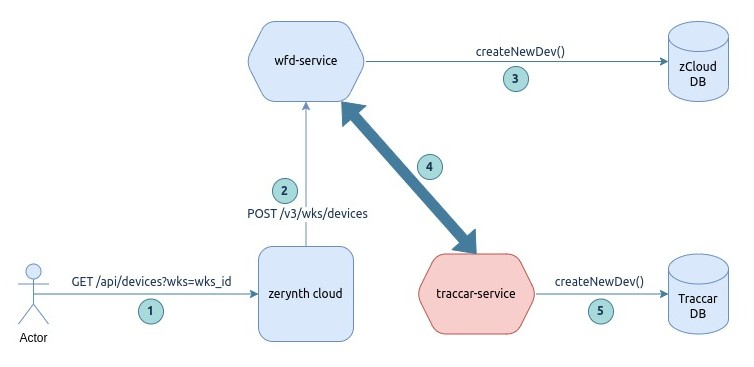
\includegraphics[scale=0.6]{images/dev_create.jpg}\\ 
\textit{Figura 4.4: Creazione di un nuovo device}
\end{center}

\subsection{
Modifica del microservizio wfd}
E' stato necessario modificare il servizio di zerynth per poter creare un oggetto nel database in traccar, dunque inizialmente ho dovuto individuare il punto in cui veniva effettuata la creazione del device. Il servizio, interamente scritto in golang, era composto da una funzione \texttt{createNewDevice()} che invocava un'ulteriore funzione chiamata \texttt{storeDevice()}. In questa parte di codice veniva eseguita a tutti gli effetti la query per memorizzare i dati del nuovo device nel database.\\
Una deduzione ovvia di questa fase è che se la query al database dovesse fallire per un qualsiasi motivo, allora la creazione del device in traccar non dovrebbe avvenire. Per implementare questo requisito, sia la query al database sia la richiesta post al servizio di traccar, sono state inserite all'interno di una \textit{transaction}. In questo modo è garantito che se il salvataggio al database non dovesse andare a buon fine, allora la richiesta di creazione di un nuovo device all'interno di traccar non verrebbe stata effettuata.
\newpage
\begin{minted}{go}
	err := p.db.RunInTransaction(func(tx *pg.Tx) error {
		err := tx.Insert(device) 
		//controlli di errore
		wks, err := p.GetWksIdOfDevice(device.ID)
		//controlli di errore
		resp := traccar_post(device, wks)
		if resp == nil {
			return errorsZDM
		}
		return nil
	})


\end{minted}


\noindent Come si può osservare da questo stralcio di codice estratto dalla funzione chiamata \texttt{storeDevice()}, sia l'inserimento dei dati all'interno del database sia l'invocazione del metodo che esegue la richiesta HTTP di tipo post del device appena creato sono all'interno della \texttt{RunInTransaction()}.\\
E' importante sottolineare che in queste righe di codice sono state omesse alcune parti, come ad esempio i vari controlli sugli errori provocati dalle varie richieste.\\
Prima di effettuare la post viene eseguita una funzione che recupera il workspace\_id relativo alla workspace alla quale il device in questione è stato aggiunto. Questa funzione che ho implementato esegue una query al database all'interno di traccar per ottenere un entità di tipo \texttt{Fleet} che rappresenta il fleet in zCloud a cui il device appartiene. Un fleet ovviamente, deve appartenere obbligatoriamente ad una workspace e questo fleet ottenuto dall'interrogazione del database di zCloud possiede dei metodi, tra i quali \texttt{getWksID()} tramite il quale è possibile risalire alla workspace a cui il device è stato appena aggiunto.\\
Adesso, per concludere questa sezione, entrerò maggiormente nel dettaglio della funzione \texttt{traccar\_post()}, essa infatti si occupa di effettuare la chiamata al servizio di traccar per permettere il salvataggio del nuovo dispositivo e prende come parametri il device e il workspace\_id di della workspace a cui esso appartiene. Questo servirà nella fase in cui l'utente accederà a traccar, e dovrà visualizzare sull'interfaccia solo i device che appartengono alla workspace che l'utente sta utilizzando in quel momento. Questa funzione infatti deve comporre il payload in Json strutturato in modo adeguato con i dati che appartengono al dispositivo, come raffigurato in figura 4.4.1, ed effettuare la richiesta post all'api \texttt{http://traccar-service:8082/api/devices}.

\begin{minted}{json}
{
   "id":0,
   "attributes":{},
   "uniqueId":"dev_id",
   "name": "name",
   "groupId": "group_id",
   "staus":"offline",
   "lastUpdate":"dd/mm/yyyy HH:MM:SS",
   "positionId":0,
   "geofenceIds":[],
   "phone":"",
   "model":"",
   "category":"",
   "contact":"",
   "disabled":false
}

\end{minted}

\noindent Prima di eseguire questa richiesta però bisogna chiarire un'ulteriore passaggio, ovvero la gestione della creazione delle workspaces. Infatti come è stato deciso in fase di analisi e studio dell'intero sistema, una workspace è rappresentabile in traccar come un gruppo che non possedesse gruppi parent. Per realizzare questo schema strutturale quindi, prima di inserire il dispositivo all'interno del database di traccar, è necessario assicurarsi che il gruppo in traccar che rappresentasse la workspace in cui il device era inserito all'interno di zCloud esistesse già. A questo punto abbiamo due casi possibili, se il gruppo dovesse esistere allora viene recuperato il suo id ed inserito all'interno del campo "groupId" del Json precedente, altrimenti è necessario creare un gruppo in traccar che possiede come campo "name" il workspace\_id della workspace desiderata. Vediamo adesso nello specifico le parti di codice che eseguono questi passaggi.\\

\begin{minted}{go}
func traccar_post(device *Device, wks string) *http.Response {
	id := exists_group(wks, device.AccountID)
	if id == 0 {
		id = create_group(wks, device.AccountID)
	}
    tdev := traccar_dev{
		Id:          0,
		Attributes:  nil,
		GroupId:     id,
		Name:        device.GetName(),
		UniqueId:    device.GetID(),
		Status:      "",
		LastUpdate:  "",
		PositionId:  0,
		GeofenceIds: nil,
		Phone:       "",
		Model:       "",
		Contact:     "",
		Disabled:    false}

	client := http.Client{}
	body, _ := json.Marshal(tdev)
	req, err := doRequest("POST", "/api/devices", payload(tdev))
	}
\end{minted}

\noindent Qui sopra è mostrato uno "sketch" del codice di questa funzione. In particolare, osservando meglio la prima parte, si può notare una chiamata ad \texttt{exists\_group()}, una procedura che restituisce il valore del'id del gruppo di traccar relativo alla workspace di zCloud, oppure 0 nel caso in cui il gruppo non esista. Per ottenere l'id del gruppo, la funzione esegue una richiesta post alla api di traccar \texttt{/api/groups?wks=wks\_id}, in questo modo il device potrà essere inserito all'interno di tale gruppo. E' bene specificare però che lato traccar-service è stato necessario effettuare alcune modifiche, infatti l'entrypoint \texttt{/api/groups} non elabora di norma il parametro "wks". Dunque la modifica che ho dovuto apportare ha interessato la classe \texttt{SimpleObjectResource()} in quanto essa è superclasse di \texttt{GroupResource()}, ed inoltre possiede un metodo che ha il compito di risolvere le richieste get da parte dei client\footnote{In realtà non gestisce tutte le richieste get, bensì essa fornisce un metodo base per le richieste get, e tutte le classi che si registrano ad una api ed estendono questa classe hanno la possibilità di usufruirne. Ad esempio la classe \texttt{deviceResource()} non estende la classe \texttt{SimpleObjectResource()} di conseguenza possiede una gestione delle richieste get alla api \texttt{/api/devices} appropriata.}. In questa parte del codice di traccar ho implementato una parte di codice che effettua un controllo sul parametro "wks", nel caso in cui sia non nullo, si procede con la chiamata ad un metodo, realizzato da me, presente in \texttt{dataManager()} che esegue una query al database di traccar, così da ottenere il gruppo che possiede il campo "name" uguale al workspace\_id passato come parametro. \\
Successivamente, osservando il codice, se il gruppo non dovesse esistere allora viene invocata la \texttt{create\_group()} che effettua una richiesta post a traccar all'api relativa ai groups con questo payload:
\begin{minted}{json}
{
   "id":0,
   "name": "wks_id",
   "group_id":0,
   "attrtibutes": {}
}

\end{minted}

\noindent Viene dunque inserito il workspace\_id all'interno del campo "name", come accennato in precedenza.\\
Ecco in figura 4.5 la presentazione grafica della comunicazione tra wfd-service e traccar-service. 
\newpage
\begin{center}
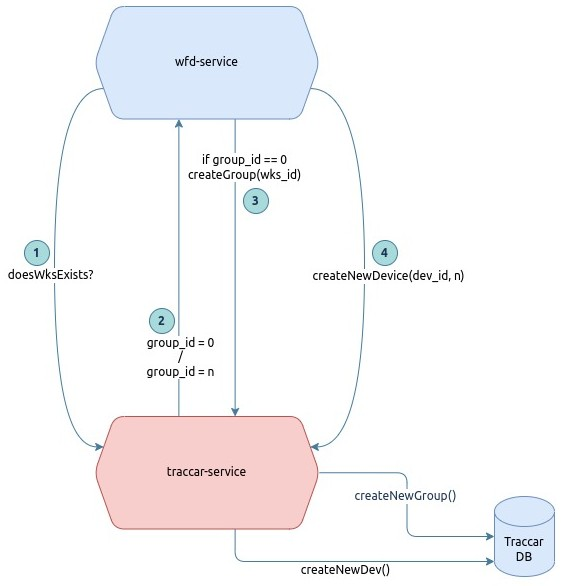
\includegraphics[scale=0.5]{images/wfd_traccar.jpg}\\ 
\textit{Figura 4.5: Interazione traccar e wfd}
\end{center}


\subsection{ 
Filtro dei device}
Per completare questa sezione correttamente, ho dovuto affrontare un ultimo problema, ovvero come restituire le informazioni corrette al client che intende visualizzare i device di una specifica workspace. Per fare ciò, una volta individuata la classe che si occupava di gestire la richiesta alla api, chiamata \texttt{DeviceResource()}, è stato indispensabile capire come modificarla correttamente per adempiere allo mio scopo.\\
Quando un utente si collega a traccar, il client effettua le chiamate api per inizializzare l'interfaccia, e tra queste chiamate vi è la richiesta get all'entrypoint \texttt{/api/devices}, che serve ad ottenere tutti i device\footnote{In realtà può essere anche invocata una richiesta per ottenere un solo o un sottoinsieme di device, indicando nella URL tutti gli uniqueId, ma è bene notare che anche in quel caso, essendo stata modificata la base url, la richiesta risulterà comunque essere: \texttt{/api/devices?wks=wks-dhwu98\&uniqueId=imei}, filtrando comunque tutti i device prima per workspace\_id e poi per uniqueId.} che appartengono all'utente.\\
Il primo cambiamento dunque è stato lato client, infatti la base url della richiesta all'entrypoint \texttt{/api/devices} doveva essere modificata, inserendo nella query un parametro che contenesse l'id della workspace desiderata. Per questioni relative al tempo l'id della workspace è stato inserito come costante, ma di fatto, non viene cambiata di molto la sostanza di questa funzionalità, in quanto basterebbe reperire il workspace\_id tramite NGNIX, analizzando la query o inserendolo come una informazione aggiuntiva in un campo header custom, dopo la richiesta da parte dell'utente. Di conseguenza l'url risultante è:\par\medskip
\texttt{http://traccar.zerynth.localhost/api/devices?wks=wks-hwb7hsoisa}\par\medskip

A questo punto il server avrebbe dovuto codificare la query e ottenere l'id della workspace e filtrare i device in base al workspace\_id. Questo è implementato all'interno di \texttt{DeviceResource()}, in cui se nella query è presente il parametro "wks" allora viene invocato un metodo che ho implementato all'interno di \texttt{ZdataManager()} chiamato \texttt{filter\_devices()}, che, data una workspace\_id, filtra i dispositivi restituendo solo quelli che appartengono a quella workspace. Per far ciò questa funzione \texttt{filter\_device()}, effettua una query al database in traccar realizzata nel seguente modo:

\begin{minted}{postgresql}
SELECT tc_devices.* 
FROM tc_devices INNER JOIN tc_groups ON tc_groups.id = tc_devices.groupid 
WHERE tc_groups.name = :wksId
\end{minted}

\noindent restituendo così tutti i device corretti.
\subsection{
Osservazioni sulle complicazioni emerse}
Inizialmente il primo tentativo che è stato fatto aveva come obiettivo evitare di duplicare l'entità dei device sul database di traccar. Questa prima soluzione però ha fatto emergere diverse problematiche, in primis riguardanti le geofences e di conseguenza anche le notifications. Infatti le geofences sono collegate strettamente ai device nel database, tramite una chiave secondaria, e riuscire a sostituire questa connessione non risulta essere semplice. Dunque è stato optato per la soluzione attuale, in quanto il tempo necessario per implementare il sistema di connessione tra le varie entità non sarebbe stato poco, inoltre non era da escludere che le idee proposte per risolvere questo problema avessero comunque fallito con una buona percentuale.\\ In generale è comunque una soluzione buona, pur duplicando le entità su due database diversi, garantisce comunque un ottimo livello di stabilità del sistema a discapito di un overhead in termini di spazio e tempo.\\
E' doveroso evidenziare che in questa parte è stata volutamente tralasciata la gestione dei fleet, in quanto si mostra molto simile a ciò che è stato fatto per i device e per le workspaces. In generale è ovvio che per uno sviluppo futuro della piattaforma sarà necessario implementare anche questa parte.


\chapter{
Integration test}
Per avere la certezza che tutto il sistema fosse stato correttamente integrato, è stata realizzata una suite di test per verificare, le funzionalità principali che il sistema integrato dovrebbe. Per testare il sistema è stata utilizzata la libreria di pytest, e quindi l'intera parte di integration test è stata scritta in python.\\
I punti principali che ho dovuto verificare sono stati:
\begin{itemize}
\item Verificare che il redirect del login avvenga correttamente, e che quindi che venga creato un utente su traccar;

\item Verificare che i dati che i dispositivi inviano a traccar siano correttamente salvati all'interno di zStorage;

\item Verificare che i device siano correttamente autorizzati e autenticati;

\item Verificare che la creazione di un device avvenga correttamente, con la creazione di un device copia nel database di traccar.
\end{itemize}

La suite di test genera un report in html in cui vengono riportati tutti gli errori riscontrati nell'esecuzione dei test. Alcune funzioni erano già fornite da Zerynth e quindi nel corso di questo capitolo non entrerò troppo dentro i dettagli implementativi.

\section{
Test del login}
Il test del login consiste nel verificare che un utente che è già registrato su zCloud riesca ad accedere ai contenuti di traccar correttamente. Per effettuarlo viene simulata una richiesta di con le credenziali di un utente già registrato, e poi una volta ottenuta la conferma che l'utente esiste su zCloud bisogna controllare che sul database di traccar è stato creato un oggetto che contiene i dati di tale utente.

\begin{minted}{python}
def test_user_auth(env_api, zcloud_client):
    res = zcloud_client.internal_auth()
    assert res.status_code == 200
    j = res.json()
    env_api._x_user_info_header = res.headers["x-user-info"]
    user = env_api._x_user_info_header.split(";")[0]
    r = requests.get("http://traccar.zerynth.localhost:8082/api/session", 
    headers={"x-user-info":env_api._x_user_info_header},auth=(user, user))
    
    assert r.status_code == 200
    j = r.json()

    assert "name" in j
    assert j["name"] == users
\end{minted}

\noindent Il primo assert presente all'interno di questo codice serve a verificare che l'utente è correttamente registrato sulla piattaforma di zCloud. Successivamente, abbiamo una richiesta ad un entrypoint di traccar e subito dopo vi sono altri tre assert. Il primo di questi tre assicura che traccar restituisca correttamente l'utente richiesto,e quindi che l'oggetto è stato adeguatamente salvato sul database di traccar. Gli ultimi due assert servono per una maggiore sicurezza, e per verificare che traccar abbia memorizzato in modo giusto i campi all'interno della tabella dell'istanza, andando a controllare gli attributi presenti all'interno del Json restituito dal server di traccar.


\section{
Test del device}
Per accertare che il salvataggio del device avvenga correttamente all'interno del database di traccar sono indispensabili due passaggi, la creazione del device all'interno di una workspace in zCloud e la richiesta dei dati del device appena creato da traccar passando come parametro il suo device\_id. Ecco qui di seguito il codice realizzato per fornire questa funzionalità.

\begin{minted}{python}
def test_device_in_traccar(zcloud_client, env_api, zdm_v3_client):
     r = zdm_v3_client._post("/workspaces/wks-6o7yvdo8inlt/devices",
     data={
         "name": "newDev"
     })
     
     assert r.status_code == 200
     j = r.json()
\end{minted}

\noindent Qui sopra viene effettuata la creazione di un device di nome "newDev" all'interno di una workspace specifica.

\begin{minted}{python}
    res = zcloud_client.internal_auth()
    r = requests.get("/api/devices?uniqueId="+dev_id,auth=(user, user))
    assert r.status_code == 200
    j = r.json()
    dev = j[0]
    assert "name" in dev
    assert dev["name"] == "newDev" 
\end{minted}

\noindent Anche in questo caso abbiamo tre assert, in cui il primo ci garantisce che il device esista anche all'interno di traccar e che quindi sia stato correttamente creato anche nel database del servizio di tracking. Gli ultimi due sono essenziali per verificare che il device abbia i campi corretti, come ad esempio quello del nome.


\section{
Test dello storage}
In questo test l'obiettivo è stato quello di assicurare che i dati che un device invia al servizio traccar, siano correttamente salvati all'interno di zStorage. Per far ciò viene simulato un device che invia dei dati fittizi tramite protocollo osmAnd a traccar, e successivamente viene prelevato l'ultimo dato inserito all'interno di zStorage da quel device e si controlla che il tag ed il payload siano quelli attesi.


\begin{minted}{python}
  r = zstorage_client._get("{0}/data?size=1&device={1}",
                                     workspace_id, device_id)  
   
  assert r.status_code == 200
  resp = r.json()       
  res = resp["result"]

  assert res[0]["tag"] == "latlon"
  assert res[0]["device_id"] == "dev-6oboztcifcox"
  assert res[0]["payload"]['latitude'] == 41.897

  t = my_time(res[0]["timestamp_device"])
  
  assert t is not None
  assert t > start 
\end{minted}


\noindent Questa parte di codice viene eseguita dopo che il device ha comunicato il payload a traccar, infatti una volta effettuata la richiesta dei dati del device in questione da zStorage, una serie di parametri vengono controllati, come ad esempio lo status-code della richiesta, e che quindi essa sia andata a buon fine, il tag del device che deve corrispondere alla stringa "latlon", l'id del device che deve corrispondere a quello del device che in precedenza ha inviato il payload id dati, ed infine il timestamp, che dev'essere superiore al tempo di inizio del test, in modo tale da essere certi di non recuperare un dato che era già presente all'interno di zStorage in precedenza.

\section{
Test dell'autenticazione del device}
Infine troviamo quest'ultimo test, in cui il compito è stato quello di confermare che il device fosse correttamente autorizzato prima di accettare la ricezione dei dati.

\begin{minted}{python}
  resp = zdm_v3_client._get(
      "/workspaces/{0}/devices/{1}/events?type=authentication&size=1",           
      env_api.workspace_id,env_api.device_id)
  assert resp.status_code == 200
\end{minted}


\noindent Viene effettuata la richiesta all'entrypoint di zCloud per verificare se quel device sia stato correttamente autorizzato dalla piattaforma per utilizzare le risorse presenti sul cloud, e per far ciò si verifica lo status code della response della richiesta.

\section{
Ulteriori modalità di testing}
Per testare ulteriormente l'integrazione del sistema ho realizzato un client in golang che simula un invio dei dati al server di traccar, con una frequenza stabilita. Questa simulazione che ho realizzato è stata utile in fase di testing ma anche e soprattutto in fase di sviluppo, per monitorare e debuggare i vari passaggi che venivano implementati. Il client è quindi costituito da un ciclo for che effettua una richiesta post, utilizzando il protocollo osmAnd al servizio di traccar. Esso invia dati riguardanti la sua posizione e il suo token indispensabile per l'autenticazione.\\
Si visualizza quindi sull'interfaccia il device in movimento, e nella demo finale ho preparato anche delle notification ed una geofence, in modo tale che nel momento in cui il device entri nella geofence, traccar invia all'utente una notifica dell'evento, come raffigurato in figura 6.1-2.\\
\begin{center}
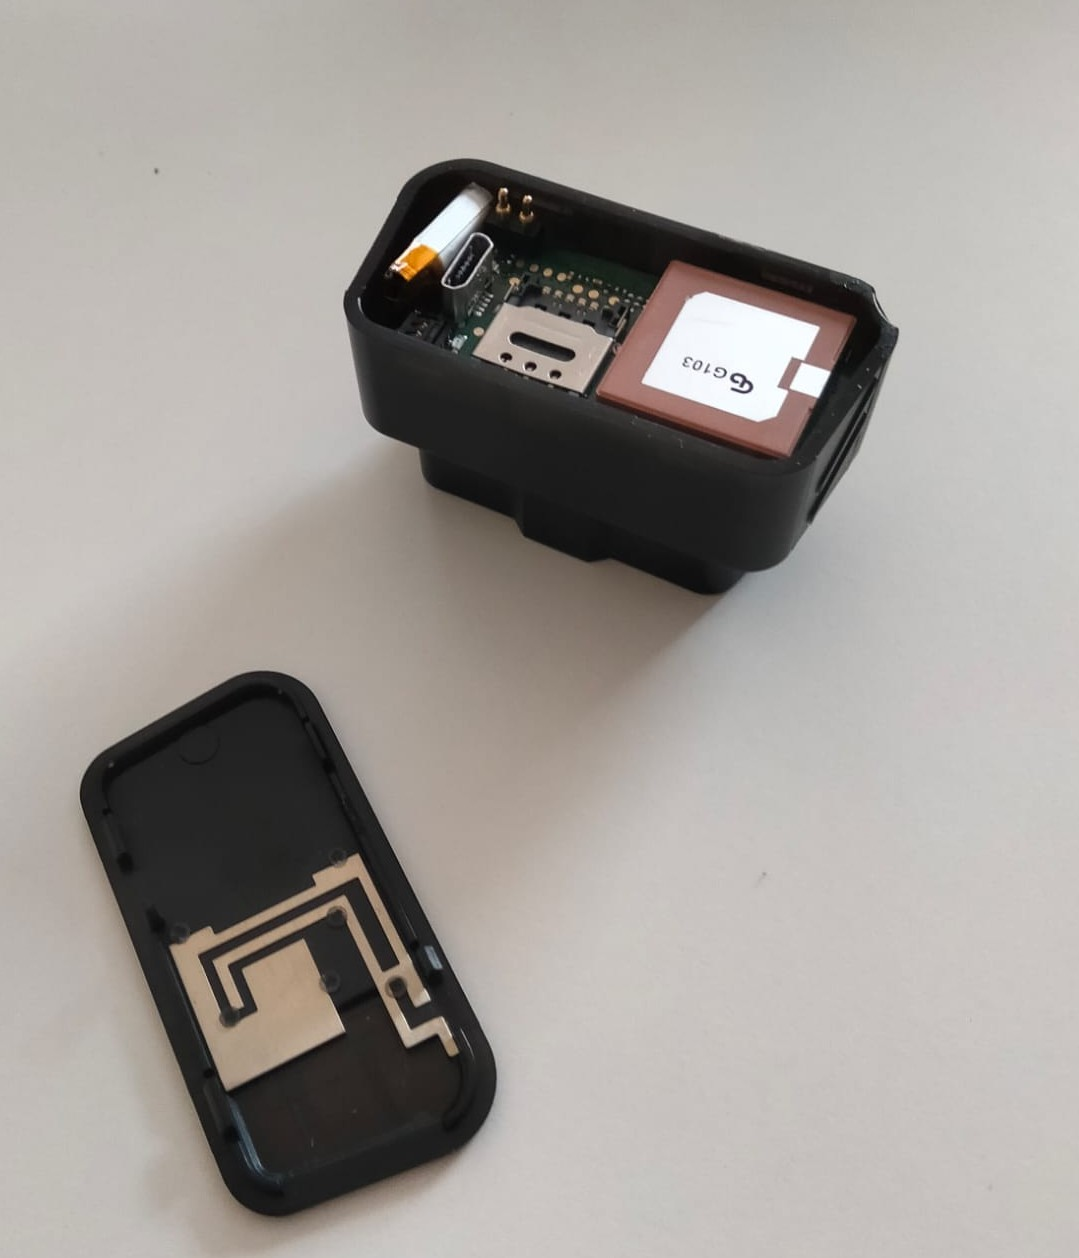
\includegraphics[scale=0.2]{images/teltotest.jpeg}\\ 
\textit{Figura 5.5: Dispositivo di test Teltonika}
\end{center}

Il passo successivo sarebbe stato quello di testare l'intero sistema integrato non in locale bensì in ambiente di test e con un device reale ed in figura 5.5 vi presento un esempio di un possibile dispositivo di testing che utilizza un protocollo appartenente alla casa produttrice chiamato TeltonikaProtocol, compatibile con traccar.\\


\chapter{
Conclusione}
In conclusione l'intero progetto è stato terminato con un buon risultato, mi ritengo nel complesso soddisfatto dell'integrazione del sistema, soprattutto per le numerose nozioni nuove che ho appreso.\\
Durante la simulazione finale si può osservare come tutte le componenti funzionano correttamente, qui di seguito illustro come ho eseguito la demo finale.

\section{
Demo finale}
L'ultima parte del progetto era ovviamente dedicata a verificare il funzionamento di tutte le componenti traccar integrate a zCloud. Per far ciò ho dovuto come prima cosa inizializzare l'ambiente, e quindi creare una workspace in zCloud e dopo creare all'interno di essa un device. Nella demo sono stati creati ben tre device come mostrato nell'immagine 6.1.



\begin{center}
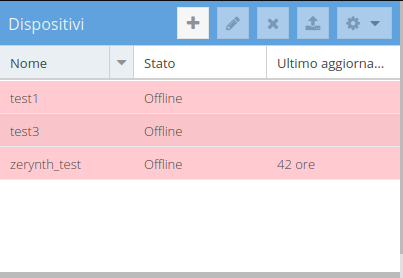
\includegraphics[scale=0.53]{images/dev.png}\\ 
\textit{Figura 6.1: Lista dispositivi}
\end{center}

Successivamente è stata creata una geofence ed una notification, entrambe poi associate al dispositivo "zerynth\_test". 

\begin{center}
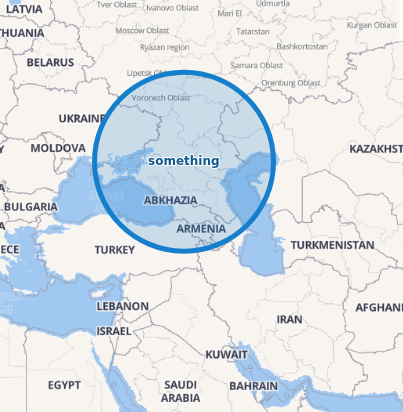
\includegraphics[scale=0.6]{images/geofence.png}\\ 
\textit{Figura 6.1-1: Creazione di una geofence}
\end{center}


Come mostrato in figura 6.1-1 la geofence è stata posizionata sulla mappa in modo tale da poter verificare il corretto funzionamento delle notifications. Infatti una volta avviata la simulazione il device "zerynth\_test" sarebbe entrato nella geofence e quindi sia l'alert che la notification sarebbero stati attivati.
\\
\begin{center}
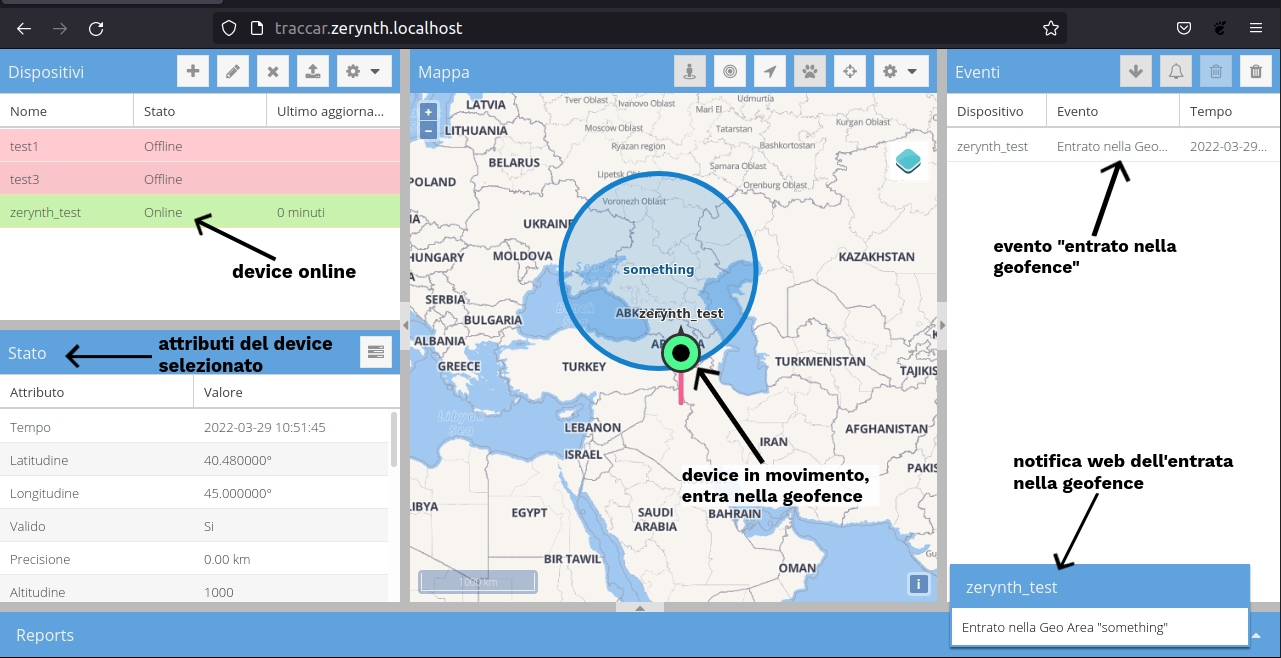
\includegraphics[scale=1.5]{images/interfaccia_completa.jpg}\\ 
\textit{Figura 6.1-2: Interfaccia finale}
\end{center}

In figura 6.1-2 è mostrata il risultato finale in cui tutte le componenti funzionano correttamente, a sinistra vengono elencati tutti i device presenti nella workspace richiesta dal client, ed in verde quelli che sono attualmente online. In basso a sinistra abbiamo invece tutti gli attributi che il device selezionato invia al server di traccar, sia standard che custom mentre a destra abbiamo la sezione degli eventi e delle notifiche.\\
Per quanto riguarda i report, nella figura 6.1-3 ne è visualizzato un esempio.

\begin{center}
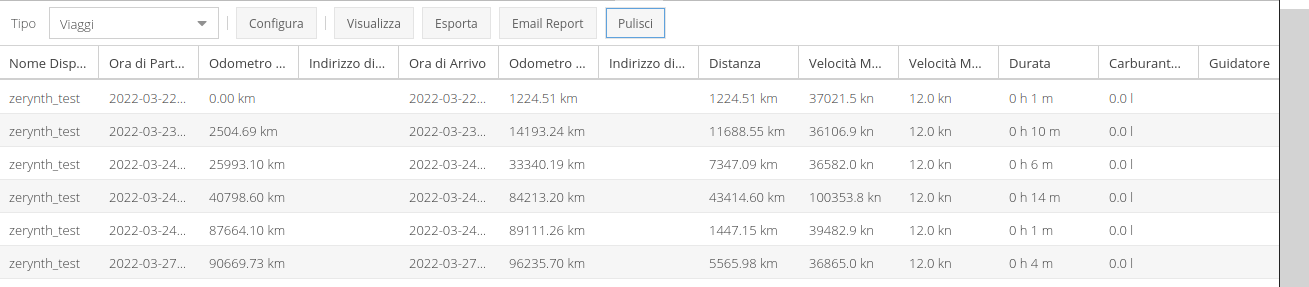
\includegraphics[scale=0.3]{images/reports.png}\\ 
\textit{Figura 6.1-3: Report di un dispositivo}
\end{center}

In questo caso vengono visualizzati i report riguardanti i viaggi del dispositivo, e quindi tutte le informazioni riguardanti la durata e le distanze.


\section{
Critiche e possibili miglioramenti}
Il lavoro finale che ho realizzato presenta ovviamente delle criticità, che lasciano spazio a miglioramenti del codice, specialmente per renderlo maggiormente estendibile, e in generale per migliorarne ad esempio alcune caratteristiche come vederemo qui di seguito.\\

\subsection{
Modularità}
Un punto essenziale per comprendere quanto un progetto sia realizzato ottimamente è la modularità, e di conseguenza quanto un software sia effettivamente estendibile con altri moduli ad esempio, o sia facile da manutenere. In questo probabilmente il sorgente che ho rilasciato come definitivo per la fase di testing presenta alcune lacune.\\
Prendendo come esempio la gestione dell'autenticazione dello user, è facile notare come sarebbe stato decisamente meglio sviluppare una nuova classe, chiamata ad esempio \texttt{ZsessionResource()} in cui veniva implementato un altro entrypoint adatto all'autenticazione per gli utenti che provenissero da zerynth.  Questo avrebbe decisamente portato ad una migliore modularità del codice e soprattutto lo avrebbe reso molto più leggibile. Invece uno dei problemi principali nella soluzione portata avanti nel progetto è quello di togliere una funzionalità base di traccar sovrascrivendo la mia parte di codice, e tale funzionalità magari avrebbe potuto rivelarsi utile per uno sviluppo futuro (ad esempio un superuser che vuole poter accedere come admin). Inoltre re-implementando questa classe, un eventuale aggiornamento del codice di traccar renderebbe molto pericoloso effettuare eventuali "merge".\\
Ovviamente la registrazione di un nuovo entrypoint e quindi di una nuova classe, necessita di competenze adeguate, e avrebbe richiesto sicuramente molto più tempo di quello che era a nostra disposizione per realizzare un progetto funzionante.

\subsection{
Gestione delle entità}
Un particolare difetto del mio progetto è l'isolamento delle api dall'esterno. Infatti il funzionamento corretto dell'interno sistema dovrebbe essere quello descritto nelle pagine precedenti, più precisamente in figura 4.4, in cui l'utente, per poter creare un device ad esempio, effettua il login sulla piattaforma di zCloud e quindi crea il device virtuale e di conseguenza verrà successivamente creata una sua copia sul database di traccar. Nella mia implementazione vi è però un problema, in quanto le api fornite da traccar sono disponibili anche all'esterno. Pertanto nonostante si possa comunque impedire all'utente di creare device (o gruppi) dall'interfaccia, rimuovendo fisicamente i buttons, rimane il problema delle api. Infatti basterebbe che l'utente effettui le richieste strutturandole in un modo preciso (e quindi ad esempio inserendo il cookie) e potrebbe essere in grado di creare o eliminare i device dal database di traccar.\\
Sebbene questo potrebbe sembrare un problema lieve, in quanto un utente non vorrebbe mai modificare, alterare o in generale danneggiare un software che lui stesso utilizza, rimane comunque un problema che espone il sistema a possibili attacchi dall'esterno. Dunque potremmo considerare questa defezione come una leggera vulnerabilità che un malintenzionato potrebbe sfruttare.


\subsection{
Duplicazione delle istanze}
Un problema che ho già trattato in precedenza è la creazione di istanze di supporto nel database di traccar. Ad esempio, con la creazione di un device all'interno di zCloud, comporta la creazione di un device all'interno del database di traccar. Questo ovviamente comporta una duplicazione delle risorse create, che in generale non è l'ideale. Limitare l'uso dello spazio è un ottimo obiettivo da porsi in applicazioni e servizi cosi grandi. Nel mio caso questa era la soluzione più veloce e semplice da implementare, e che allo stesso tempo rendesse l'intero sistema molto più stabile preservando tutte le altre funzionalità base che traccar fornisce.


\section{
Analisi dei punti di forza del lavoro svolto}
Sebbene molte parti sono state realizzate sovrascrivendo o aggiungendo alcune parti nel codice di traccar, in altri punti  l'integrazione delle nuove funzionalità è stata implementata con l'aggiunta di intere classi. Ne è un esempio la classe \texttt{ZdataManager()} in cui sono contenute tutte le funzioni di utility, per pubblicare sulla coda rabbitMQ, per autorizzare i device e per filtrare i device in base alla workspace; ma anche la classe \texttt{zDataHandler()}  che come già accennato in precedenza ha il compito di implementare un handler, che a sua volta gestirà le posizioni che i device stanno comunicando.\\
Ma uno di punti di forza del mio progetto è senza dubbio la possibilità da parte dei device di poter utilizzare fino a 127 protocolli diversi. Infatti tutte le funzionalità implementate in aggiunta sono state realizzate ad un "livello superiore" di astrazione, e quindi dopo che i vari decoder dei protocolli hanno effettuato la decodifica. Dunque questo permette di autenticare e autorizzare un device e permettere ad esso di scrivere i suoi dati nello zStorage a prescindere dal protocollo che viene utilizzato per inviare dati al server di traccar.

\section{
Ultime osservazioni sugli obiettivi raggiunti}
In generale mi ritengo pienamente soddisfatto del lavoro effettuato sia per come sono stati raggiunti gli obiettivi preposti, sia del percorso che ho affrontato, nel quale ho imparato a comprendere al meglio il vero funzionamento di un'architettura cloud strutturata con microservizi.\\
Mi ha particolarmente colpito come è complessa la struttura e la composizione dei diversi servizi, inoltre la possibilità di analizzare il codice di un software esistente mi ha permesso di apprendere in modo più concreto come è realizzato un codice di un software esistente, in tutte le sue componenti, codice sorgente, codice compilato, e anche il lato front-end e quindi tutta la parte relativa all'interfaccia e in generale al lato client.\\
Di certo la fase implementativa è stata quella che mi ha interessato maggiormente, e quindi risolvere tutte le complessità che si ponevano davanti, mentre, posso affermare con certezza che la complessità maggiore è stata senza dubbio quella di comprendere davvero a fondo il funzionamento di traccar, e quindi analizzare il codice per comprendere al meglio le funzionalità di ogni classe in modo da essere consapevole cosa stessi modificando e quali conseguenze avrebbe potuto comportare ogni singola riscrittura del codice. Infatti numerose volte è accaduto che intere fasi si bloccassero spesso o comunque subissero rallentamenti poiché piccole righe di codice modificate all'interno di una classe provocavano grandi effetti collaterali su funzionamenti interni del software.\\
Durante questo tirocinio ho anche appreso come possono essere utilizzati strumenti come le code rabbitMQ o la piattaforma docker e docker-compose, le suite di test per controllare funzionalità specifiche di integrazione del sistema, l'utilizzo appropriato di query per prelevare o inserire dati in un database ed infine anche come sfruttare correttamente lo stile architetturale REST, utilizzando le chiamate api in modo corretto per implementare funzionalità o testare il sistema.

\section{
Ringraziamenti}
Concludo il documento con i dovuti ringraziamenti, nei confronti dell'università che mi ha permesso di intraprendere questa opportunità, in particolar modo al professore Gabriele Mencagli che mi ha seguito durante tutto il processo di stesura della tesi. Allo stesso modo i ringraziamenti sono rivolti anche all'azienda che mi ha permesso, con le dovute precauzioni dovute alla pandemia da Covid-19, di svolgere questo tirocinio anche in presenza e a tutti coloro che ho avuto il piacere di conoscere durante questa mia piacevole esperienza. In modo particolare ringrazio Davide Neri, che in qualità di tutore aziendale, grazie alla sua disponibilità, mi ha aiutato a proseguire nel progetto superando alcune difficoltà incontrate e indicandomi la strada migliore li dove avessi incertezze sulle scelte da realizzare.


}





















\end{document}